\section{Basics of 3D Graphics}

Everything in modern computer graphics is centered around polygon meshes.
A polygon mesh is a geometric graph combined with a set of geometrical faces that together form a surface.
Typically these faces are triangles, in which case the meshes are also referred to as triangle meshes, or simply meshes.
An example of such a mesh is shown in Figure~\ref{fig:low_poly_dolphin}.

\begin{figure}[h!]
  \centering

  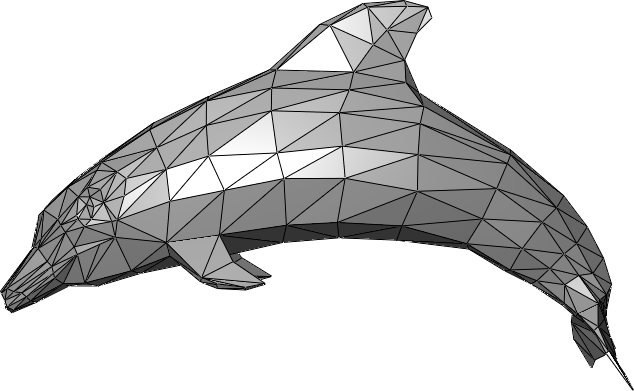
\includegraphics[width=0.5\textwidth]{figure/low_poly_dolphin.png}
  \caption{Example of a low poly triangle mesh representing a dolphin \cite{low_poly_dolphin}.}

  \label{fig:low_poly_dolphin}
\end{figure}

\newpage
Each vertex can store arbitrary data alongside its own coordinates in space.
Examples of such data include: an averaged normal of its neighboring faces, color, reflectance, bone weights and texture coordinates (a.k.a. UV coordinates).
These stored properties can then be used to help compute realistic lighting, colors, animations, and more.

Nowadays it is common to apply high-quality images to meshes, rather than just colors and lighting shades.
Applying these images can be done via a process called \textit{texture mapping} or \textit{UV mapping}, which entails designing 2D textures and mapping these onto 3D meshes using the UV coordinates of the vertices.
An example of this process can be found in Figure~\ref{fig:uv-mapping}.

\begin{figure}[h!]
  \centering
  \begin{subfigure}[b]{0.30\textwidth}
    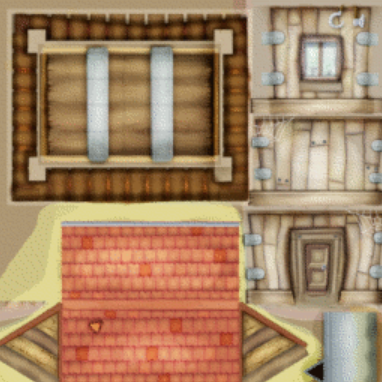
\includegraphics[width=\textwidth]{figure/uv-mapping1.png}
    \caption{House texture map.}
  \end{subfigure}
  \quad
  \quad
  \quad
  \begin{subfigure}[b]{0.30\textwidth}
    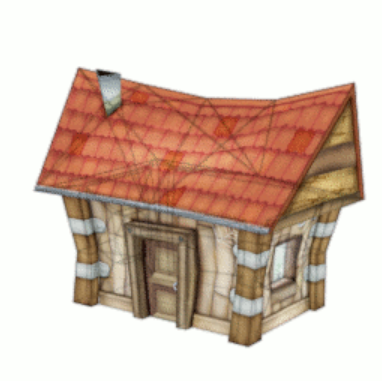
\includegraphics[width=\textwidth]{figure/uv-mapping2.png}
    \caption{Textured house mesh.}
  \end{subfigure}

  \caption{Example of UV mapping a texture map onto a model of a house \cite{house_uv_mapping}. Notice how UV coordinates are reused to apply the same texture to each pillar.}
  \label{fig:uv-mapping}
\end{figure}

Models can be future enhanced by using materials and shaders.
A material contains all the visual properties of a model except for the mesh itself.
This may include multiple constants, textures, and shaders.
Shaders are programs designed to run on GPUs and can be used to combine textures in various ways to create interesting visual effects.
The downside is that shaders are typically strongly tied to specific software or hardware, making them difficult to port.
Consequently, standard file formats for 3D models such as \textit{.obj}, \textit{.fbx}, and \textit{.gltf} have limited support for shaders.
